%  LaTeX support: latex@mdpi.com 
%  In case you need support, please attach all files that are necessary for compiling as well as the log file, and specify the details of your LaTeX setup (which operating system and LaTeX version / tools you are using).

% You need to save the "mdpi.cls" and "mdpi.bst" files into the same folder as this template file.

%=================================================================
\documentclass[ijfs,article,submit,oneauthor,pdftex,10pt,a4paper]{mdpi} 
%
%--------------------
% Class Options:
%--------------------
% journal
%----------
% Choose between the following MDPI journals:
%ijfs, 
%------
% article
%---------
% The default type of manuscript is article, but can be replaced by: 
% abstract, addendum, article, benchmark, book, bookreview, briefreport, casereport, changes, comment, commentary, communication, conceptpaper, correction, conferenceproceedings, conferencereport, expressionofconcern, meetingreport, creative, datadescriptor, discussion, editorial, essay, erratum, hypothesis, interestingimages, letter, meetingreport, newbookreceived, opinion, obituary, projectreport, reply, reprint, retraction, review, perspective, protocol, shortnote, supfile, technicalnote, viewpoint
% supfile = supplementary materials
% protocol: If you are preparing a "Protocol" paper, please refer to http://www.mdpi.com/journal/mps/instructions for details on its expected structure and content.
%----------
%submit
%----------
% The class option "submit" will be changed to "accept" by the Editorial Office when the paper is accepted. This will only make changes to the frontpage (e.g. the logo of the journal will get visible), the headings, and the copyright information. Also, line numbering will be removed. Journal info and pagination for accepted papers will also be assigned by the Editorial Office.
%------------------
% moreauthors
%------------------
% If there is only one author the class option oneauthor should be used. Otherwise use the class option moreauthors.
%---------
% pdftex
%---------
% The option pdftex is for use with pdfLaTeX. If eps figures are used, remove the option pdftex and use LaTeX and dvi2pdf.

%=================================================================
\firstpage{1} 
\makeatletter 
\setcounter{page}{\@firstpage} 
\makeatother 
\articlenumber{x}
\doinum{10.3390/------}
\pubvolume{xx}
\pubyear{2017}
\copyrightyear{2017}
\externaleditor{Academic Editor: name}
\history{Received: date; Accepted: date; Published: date}

%------------------------------------------------------------------
% The following line should be uncommented if the LaTeX file is uploaded to arXiv.org
%\pdfoutput=1

%=================================================================
% Add packages and commands here. The following packages are loaded in our class file: fontenc, calc, indentfirst, fancyhdr, graphicx, lastpage, ifthen, lineno, float, amsmath, setspace, enumitem, mathpazo, booktabs, titlesec, etoolbox, amsthm, hyphenat, natbib, hyperref, footmisc, geometry, caption, url, mdframed, tabto, soul, multirow, microtype, tikz
\usepackage{rotating}
\usepackage{pdflscape}
\usepackage[flushleft]{threeparttable}
\usepackage{changes}
\setremarkmarkup{(#2)}
%\usepackage[comma, sort&compress]{natbib}% Use the natbib reference package - read up on this to edit the reference style; if you want text (e.g. Smith et al., 2012) for the in-text references (instead of numbers), remove 'numbers' 
%=================================================================
%% Please use the following mathematics environments: Theorem, Lemma, Corollary, Proposition, Characterization, Property, Problem, Example, ExamplesandDefinitions, Hypothesis, Remark, Definition
%% For proofs, please use the proof environment (the amsthm package is loaded by the MDPI class).

%=================================================================
% Full title of the paper (Capitalized)
\Title{Foreign Exchange Speculation: An Event Study}

% Author Orchid ID: enter ID or remove command
%\newcommand{\orcidauthorA}{0000-0000-000-000X} % Add \orcidA{} behind the author's name
%\newcommand{\orcidauthorB}{0000-0000-000-000X} % Add \orcidB{} behind the author's name

% Authors, for the paper (add full first names)
\Author{Rob Hayward $^{1,\dagger,\ddagger}$}

% Authors, for metadata in PDF
\AuthorNames{Rob Hayward}

% Affiliations / Addresses (Add [1] after \address if there is only one affiliation.)
\address{$^{1}$ \quad University of Brighton; rh49@brighton.ac.uk}

% Contact information of the corresponding author
\corres{Correspondence: rh49@brighton.ac.uk; Tel.: +44-1273-642-586}

% Current address and/or shared authorship
\firstnote{Current address: Lewes Road, Brighton BN2 4AT} 
%\secondnote{These authors contributed equally to this work.}
% The commands \thirdnote{} till \eighthnote{} are available for further notes

% Simple summary
%\simplesumm{}

% Abstract (Do not insert blank lines, i.e. \\) 
\abstract{Does speculation facilitate price discovery or instability?  If it is price discovery, it is beneficial and should be encouraged; if it is instability, welfare is enhanced by its reduction. This paper seeks to distinguish between these two characteristics by analysing those times when speculation in the foreign exchange market is most extreme.  A series of event studies are conducted on the extremes of speculative activity and speculative sentiment. If speculation is noise,  extreme sentiment and extreme positions should lead to overshooting and increase risk of subsequent reversals. The finding that speculative extremes do not provide information about subsequent returns implies that speculation is part of the process of price discovery and that efforts to reduce it would reduce the informational efficiency of financial markets.}

% Keywords
\keyword{Foreign Exchange ; Speculation; Event-study.}

% The fields PACS, MSC, and JEL may be left empty or commented out if not applicable
%\PACS{J0101}
%\MSC{}
%\JEL{}

%%%%%%%%%%%%%%%%%%%%%%%%%%%%%%%%%%%%%%%%%%
% Only for the journal Applied Sciences:
%\featuredapplication{Authors are encouraged to provide a concise description of the specific application or a potential application of the work. This section is not mandatory.}
%%%%%%%%%%%%%%%%%%%%%%%%%%%%%%%%%%%%%%%%%%

%%%%%%%%%%%%%%%%%%%%%%%%%%%%%%%%%%%%%%%%%%
% Only for the journal Data:
%\dataset{DOI number or link to the deposited data set in cases where the data set is published or set to be published separately. If the data set is submitted and will be published as a supplement to this paper in the journal Data, this field will be filled by the editors of the journal. In this case, please make sure to submit the data set as a supplement when entering your manuscript into our manuscript editorial system.}

%\datasetlicense{license under which the data set is made available (CC0, CC-BY, CC-BY-SA, CC-BY-NC, etc.)}

%\setcounter{secnumdepth}{4}
%%%%%%%%%%%%%%%%%%%%%%%%%%%%%%%%%%%%%%%%%%

\begin{document}
\section{Introduction}
\added{Speculation can be stabilising or destabilising.} If speculation is based on information it is a stabilising force, providing liquidity and helping to ensure that markets swiftly find equilibrium. \citet{KeynesHedge} and \citet{HicksHedge} \deleted{for example} emphasise the role that speculation plays in facilitating financial market transactions \added{by providing liquidity that allows hedgers and other market participants to swiftly find counterparties without the need for large prices concessions.} Speculators offer a service for a fee that is determined by the return on their activity.  \replaced{\citet{FriedmanPositive} argued that even where there are a mixture of infomed and unnformed speculators, the informed woudl tend to buy when prices were below intrinsic value and sell when above, making profits, stabilising the market and driving the loss-making uninformed speculators out of business.}{While speculators may be trading on information or noise, informed speculators will tend to drive out the uninformed noise-traders according to \citet{FriedmanPositive}.} \deleted{However, the later} \citet[p. 101]{Keynes1936} \added{also had a later, more negative view of speculation.  Here he} regarded speculation as a myopic, sentiment-driven activity, dominated by the desire to ``beat the gun'' or  ``outwit the crowd''\added{. Uninformed speculators may now dominate} and \citet{Delong1990noise} provide a model \deleted{of cases} where speculative noise provides a constraint on informed traders benefiting from their knowledge. Now speculation is an uninformed and destabilising force.  \added{We have therefore two concepts of speculation: one that is random and disruptive and one that is informed and beneicial in its provison of liqidity.

The debate about the relative merit of these two concepts of speculation continues to the current era where there has been much discussion over the role that speculation played in the boom and bust of commodities prices in the period between 2006 and 2007.  A common story that has encouraged Congressional investigation says that wild speculation drove oil and other commodities prices well above their fundamental value causing harship for commodity consumers and a subsequent collapse that was equally disruptive for the producders.  \citet{PindyckSpec} show a broad movement of commodities prices not linked to fundaments that they argue is caused by speculation.  \citet{TangSpec} suggest that this disruption was exacerbated by speculation on commodity indices.  However, \citet{ScottSpec} do not find a link between speculative positions and excess price movements in commodities and \citet{Jacksspec} documents a long history of attacks on speculation following price volatility.}

This paper evaluates the relative importance of these two concepts of speculation by investigating the relationship between the intensity of speculation and the weight of speculative positions relative to subsequent movement of foreign exchange prices.\footnote{\label{FX}The foreign exchange market is chosen for this study because it is the largest and most liquid financial market in the world.  The latest survey taken by the Bank for International Settlements (BIS) in April 2016 estimated average daily turnover at \$5.1trn with average daily spot transactions of \$1.7trn See \citet{BISFX2016}.  The cost of trading in this market, when measured in terms of the size of the bid-ask spread, is extremely low. An analysis by \citet{Steely2013} of the bid-ask spreads for USD-JPY, GBP-USD and EUR-USD for the period January 2001 to 2005 finds that the average spread for each is 0.342\%, 0.305\% and 0.326\% respectively.  This would be the cost for a round-trip (buying and selling immediately).}  \added{The intenisty of speculation is measured with the use of option risk-reversal skew.  As these become more extreme it signals that expectations of buyers and sellers in the foreign exchange options market have diverged significantly from the forward rate.  Weight of speculative positions is measured by the net long or short of speculative accounts in the futures market. If the movement of prices towards equilibrium, \emph{price discovery} is facilitated by order flow from informed traders (as has been asserted theoetically by \citet{Glosten1985Bid} and \citet{Kyle1985Continuous} while being demonstrted empirically by \citet{Lyons1995Microstructure} and \citet{Evans2002Order} and \citet{rime2010exchange}, speculative sentiment and positions would be part of the price discovery process if informed and would disript this process if not. Therefore,}if speculators are informed their activity drives exchange rates towards equilibrium and prices should follow a random walk after these extremes \added{of speculative sentiment or position}; if speculators are uninformed and their activity can be regarded as noise, the most extreme speculative sentiment and the time when speculators have the greatest weight in the market should correspond with the greatest deviation of prices from fundamental value, when reversals are most likely to take place.  

The rest of the paper proceeds as follows:  Section Two presents the framework of informed and uninformed speculation; Section Three talks about the measurement of speculation and the event study method; Section Four reviews the evidence; Section Five concludes. 

\section{Informed and uninformed speculation}
Speculation plays an important part in several areas of financial economics.  However, there is no clear, unambiguous theory of speculation.  Speculation is frequently associated with the term trading and the provision of liquidity, but trading is broader as it encompasses financial investment while liquidity provision is really market-making. Speculation and trading can be categorised as being informed or uninformed. Those trading without information are frequently called \emph{noise-traders} or \emph{liquidity traders}.  However, the terms are not fixed and  \citet[p. 1]{GortonNoise} categorise noise-traders as all those trading in markets for ``non-information-based reasons''.  See \citet{Ramiah201589} for a recent review of the noise-trader literature. 

The comparison of informed and uninformed traders is a central component of microstructure research.  At the heart of the \citet{Kyle1985Continuous} model of market-making is the interaction of orders from the informed and the uninformed.  On the assumption that uniformed orders arrive in a random fashion, the weight of orders reveals the direction of private information and should encourage adjustment of the bid-ask spread as part of the process of price discovery.  \citet{glosten1985bid} presents a model where the bid-ask spread is a function of adverse selection, being caused by the risk that orders come from informed traders.  

\citet[p.529]{BlackNoise} asserted that the interaction of informed and uninformed activity was essential to the smooth functioning of financial markets. Noise, he argued, was the  ``the arbitrary element in expectations''. Therefore, noise makes financial markets possible but imperfect: the more noise-traders that there are, the more liquidity and the easier it is to trade; the more noise-traders, the higher the level of inefficiency in the market and the more likely that price will be driven from fundamental value. 

Uninformed activity provides a rationale and the opportunity for trading. Unless there is a difference of opinion about value, there is no reason to exchange. Uninformed speculation can create space between price and fundamental value that can be exploited by informed speculators.  This space can encourage informed traders to pay the cost of acquiring information in the \citet{Grossman1980Impossibility} model.  There is equilibrium between the cost of obtaining information and the benefits that are expected to come from the use of the information.  

\added{More recently the debate has move towards the way that noise-trading speculators may affect welfare and how that could be contained. \citet{Tobin1982} and \citet{Tobvin} developed the argument for the eponymous transaction tax that would seek to limit the influence of exchange rate speculation.  \citet{ERW} use a series of fundamentals to show how speculation casued unwarranted devaluations during the period of the European Exchange Rate Mechanism (ERM).   \citet{Tobin3} use this experience to re-state the call for a tax to reduce speculation.  However, if speculation is informed and part of the process of price discovery this tax can be counterproductive as it will reduce liquidity and may cause evengreater volatility. This is a point made by \citet{Mayer} and \citet{McKinnon}. 

The call for a tax on speculative activity in financial markets arose again in the middle of the first decade of the new century as a result of surge in commodities prices that was experienced in the period 2005 to 2007. Focused mostly on oil but encompassing many other energy, metal and food commodities, one argument attributed the rise in prices again to speculative actvity.  See..}.

\section{Measuring speculation}
\added{It is common practice to back market expectations out of information drawn from option prices.  This is where the expectatiosn and other information goes.  Using the risk-reversal skew is a simplified version of that.}  \footnote{If the risk-reversal for a 1-month USD/CAD is quoted at 0.15-0.28\% and the implied volatility is 8.50\%, the market-maker would be willing to buy the 1-month 25 delta USD-put-CAD-call at 8.65\% and sell the USD-call-CAD-put at 8.50\%.  The dealer pays 0.15\%.  Alternatively, the dealer would sell a 25 delta call at 8.78\% and buy the USD-call-CAD-put at 8.50\%, earning 0.28\%. See \citet{Global} for a technical review. }  Therefore, the relationship between implied volatility for calls and implied volatilities for puts for the same delta and maturity strike is an indication of how much more expensive calls are relative to the equivalent put or as the market bias towards puts over calls and as an indication of market sentiment or related market positioning.  The larger the absolute level of the risk-reversal skew, the greater the relative price and, if the deviation is based on information, subsequent price action should be zero on average; if the deviation is based on noise, this movement should be reversed.  See \citet{Yan2011} and \citet{FengZhangFriesen} for some analysis of implied volatility in the equity market. 

Recording speculative activity in an over-the-counter market like foreign exchange is extremely difficult.  However, there are some exchange-traded currency derivative markets in the US, and participants in these markets are required to report their positions to the US regulators.  The Commodity Futures Trading Commission (CFTC) collect weekly information about the open positions held by private entities in the US derivative markets.   A sub-set of this information is released to the public each week as the \emph{Commitment of Traders Report} (CoT).\footnote{The \citet{cot} require traders to categorise themselves as being either commercial (C) or non-commercial (NC).  Commercial traders must have some underlying business interest in the security, commodity or instrument that they are trading.  These could be seen as natural hedgers.  Non-commercial accounts are generally considered to be speculators.  See \citet{FuturesSanders} and \citet{FuturesWang} for examples of previous use of this data in this fashion.  
 
The data used run from September 30 1998 when the data started to be released on a weekly basis and continue up to December 31 2008.  The Euro data runs from March 3 1998 to December 31 2008.  There are two gaps in the Swiss Franc data for September 14 2004 and September 21 2004.  The absence of these data seems to be a result of problems with the CFTC database.  The contracts are for EUR 100,000; GBP 62,500; JPY 12,500,000; CHF 100,000 and CAD 100,000.}  

An event study will analyse the performance of security of asset prices around an event.  In this case the event is the extreme of speculative sentiment or extreme speculative activity.  See \citet{Dolly1933} for the original version of the event study method and \citet{FamaFisherJensenRoll} for an overview of the method used in this study. 

\section{Analysis of results}
  Table \ref{tabref:RR1} records the result of the event studies that were carried out on extreme risk reversal.   For each exchange rate the second column distinguishes between extreme high and extreme low risk-reversals, the third  column identifies the number of extreme events that were recorded while the following two columns show the cumulative average returns for the whole event window (CARW) and the cumulative average returns for the event and the period after (CARA).  The windows were chosen to correspond to one day and one week of trading.  
\begin{sidewaystable}
% multirow package is required.   
%pdflandscape is required to facilitate the landscape position. 
\begin{threeparttable}
\caption{Event Study: Cumulative Abnormal Returns and Extreme Risk Reversal}
\begin{tabular}{llccccccccccccc}  
 % \hline
& &\multicolumn{6}{c}{$5^{th}$ and $95^{th}$ percentile} & \multicolumn{1}{c}{} & \multicolumn{6}{c}{$1^{st}$ and $99^{th}$ percentile}\\
 & &\multicolumn{3}{c}{1 day} & \multicolumn{3}{c}{4 day} & \multicolumn{1}{c}{} & \multicolumn{3}{c}{1 day} & \multicolumn{3}{c}{4 day} \\ 
%\cline{4 - 10} \cline{13 - 19}
& &\multicolumn{1}{ c}{N} & \multicolumn{1}{c}{CARW} & \multicolumn{1}{c}{CARA} & \multicolumn{1}{ c}{N} & \multicolumn{1}{c}{CARW} & \multicolumn{1}{c}{CARA} & \multicolumn{1}{c}{} & 
\multicolumn{1}{ c}{N} & \multicolumn{1}{c}{CARW} & \multicolumn{1}{c}{CARA}  
& \multicolumn{1}{ c}{N} & \multicolumn{1}{c}{CARW} & \multicolumn{1}{c}{CARA}  \\   
\hline
\multirow{2}{*}{EUR} 
& Hi &  87 &  0.4103* &0.1586 &87 &0.9442* & 0.1505 &&22 &0.0309 & -0.1748 &22 & 0.5781*& -0.5387*  \\ 
& Lo & 106 &-0.3313* & -0.0933 &106 &-0.0816* &-0.1991 & & 21&0.3040 &0.1820 &21 &0.7935* & 0.4377  \\
\multirow{2}{*}{JPY}
& Hi & 90 &0.4860* &0.1341 &90 &1.5158* &0.2531 & &20 &0.8227* &0.3078* &20 &2.4337* & 0.8284*  \\ 
& Lo & 90 &-0.3168 &0.0945 &90 &-1.3532* &0.1984 & &17 &-1.6990* &-0.9347* &17 &-3.6751* & -1.2556*  \\
\multirow{2}{*}{GBP}
& Hi & 96 &0.3303* &0.1903* &96 &0.8966* &0.2547 & &21 &0.5252* &0.1774 &21 &1.3131* &0.3284  \\ 
& Lo & 97 &-0.1894 &0.0312 &97 &-0.8031* &0.1500 & &24 &-0.2630 &-0.0866 &24 &-0.6660 &0.1888  \\
\multirow{2}{*}{CHF}
& Hi & 80 &0.0065 &-0.0565 &80 &0.5624* &0.1322 & &18 & -0.0022 & -0.1518 &18 &0.4887 &-0.1768  \\ 
& Lo & 75 &-0.3716* & -0.1125& 75 &-1.0071* &-0.0219 & &18 &0.0064 &0.1704 &18 &-0.8661* &0.7631  \\
\multirow{2}{*}{CAD}
& Hi & 113 &-0.0038 &-0.0489 &113 &0.1872 &-0.1951 & & 24 &-0.1081 & -0.0462 &24 &0.3935* & -0.1592  \\ 
& Lo & 97 &-0.1422* & -0.0571 & 97 & -0.2896* & 0.0035& & 26 & -0.2008 & -0.0146 &26 &0.1185 & 0.4560*  \\
\multirow{2}{*}{AUD}
& Hi & 101 &0.2539* &0.0125 &101 &0.8728* & 0.0875 &  &33 &0.5099* &0.0682 &33 & 1.1501*& 0.1046  \\ 
& Lo & 138 &-0.4384* & -0.1711 & 138 & -1.14935* & -0.2714* & &20 &-0.4334 & 0.0563 &20  & -1.7360* & 0.1914  \\
\multirow{2}{*}{EURJPY}
& Hi & 95 &-0.0504 &-0.1103 &95 &-0.0128 &-0.2579 & &23 &-0.2932 &-0.4188* &23 &-0.8203 & -1.0195  \\ 
& Lo & 97 &-0.4746* & -0.1647 &97 &-1.6757* &-0.4595 & &20 &-1.3630* & -0.6976* & 20 & -3.6849* &-1.1999*  \\
\multirow{2}{*}{EURGBP}
& Hi & 91 & 0.1544 &0.0696 &91 &0.5176* &0.0979 & &28 &0.2048 &0.1195 &28 & 0.4146 & -0.0645  \\ 
& Lo & 122 & 0.0451 & 0.0996 &122 &-0.3097* &0.2903* & & 21 &-0.07523 &-0.0780 &21 & -0.4120 &
-0.1290  \\
\multirow{2}{*}{EURCHF}
& Hi & 77 & 0.1183* & 0.0690 &77 & 0.3444* & 0.0749& & 	31 & 0.1482* &0.0739  &31 & 0.4993* 
& 0.1816*  \\ 
& Lo & 94 &-0.0344 & 0.0194 & 94 & -0.1596 &0.1952* & &24 & -0.3626* &-0.1483 & 24 & -0.7573* 
& 0.0875  \\
\hline
\label{tabref:RR1}
\end{tabular}
\begin{tablenotes}
\small 
\item Where Hi means extreme high in the risk-reversal skew and Lo means extreme low in the risk reversal skew; extreme is calculated as being equal or above the $95^{th}$ or $99^{th}$ percentile or equal or below the $5^{th}$ or $1^{st}$ percentile respectively; CARW is the cumulative abnormal return for the whole window, before and after the extreme event, and CARA is the cumulative abnormal return for the period after the event, which is the event day and the window; abnormal return is anything that is different from zero; the asterisk denotes significantly different from zero, where statistical significance is more than 95\% of 1000 means calculated from random bootstrap samples from the events are above or below zero respectively.   
\end{tablenotes}
\end{threeparttable}  
\end{sidewaystable}

As speculators become more extreme in their opinion, exchange rates are driven in the direction of sentiment. Looking down the seventh column (the 4-day CARW) reveals the average cumulative return for the period from four days before the extreme speculative sentiment to the four days after the event.   The extreme highs are those points when the risk-reversal skew is at or above the $95^{th}$ percentile.  For the whole event window (CARW), extreme highs (labelled "Hi") are associated with positive returns and the extreme lows (labelled "Lo") are associated with negative returns. In most instances these are significantly different from zero.  

That sentiment drives price appears evident from the covariance of speculative sentiment with exchange rate prices. This finding is consistent with the evidence of previous research that has used order-flow or sentiment from the likes of \citet{Evans2002Order}, \citet{FuturesSanders} and \citet{FuturesWang}. If speculation is not informed, the extreme is caused by herding or institutional features; if speculation is informed, it is facilitating the absorption of this information into the price. 

Does knowledge about the extreme at event time $t = 0$ provide information about the future returns?  If this speculation is noise, informed traders, such as real money or long-term fundamental accounts, should take advantage of the space that has been created between the price and the fundamental value and a reversal should be seen.  Whether this is the case is recorded in columns 5, 8, 11 and 14 of Table \ref{tabref:RR1}. A reversal is indicated by a significant negative reading for highs or positive reading for lows.   Looking, for example, at the four-day window in column 8, it is clear that the extreme risk reversal skew does not provide any information about future returns.  Of the eighteen cases using the $5^{th}$ and $95^{th}$ percentiles to identify extremely negative and extremely positive sentiment respectively, ten show a continuation (rather than a reversal) that is not significantly different from zero; one shows a significant continuation; five show reversals that are not significant; only two show significant reversal - EURCHF in each case.  For the more extreme event when the $99^{th}$ percentile is used, there is even less clarity.  Just over half the cases with the four-day window show a reversal (8 of 18), but only 2 of these are statistically significant. Exchange rate prices are as likely to go up as down after an extreme and there does not appear to be any information about the future from knowledge of these extremes. Extremes seem to be followed by a random walk as would be the case if the extreme were the result of information being absorbed into the price.  Figures \ref{fig:ES5} and \ref{fig:ES5} show details of a selection of the event studies.  Figure \ref{fig:ES5} is the extreme high ($99^{th}$ percentile) with a 16 day window. There is no evidence of a reversal in any of the currency units.   Figure \ref{fig:ES5} is the extreme low ($10^{th}$ percentile) with a 16 day event window.  Only the CAD shows any evidence of reversal. 

\begin{figure}
\graphicspath{{../Figures/}}
\centering
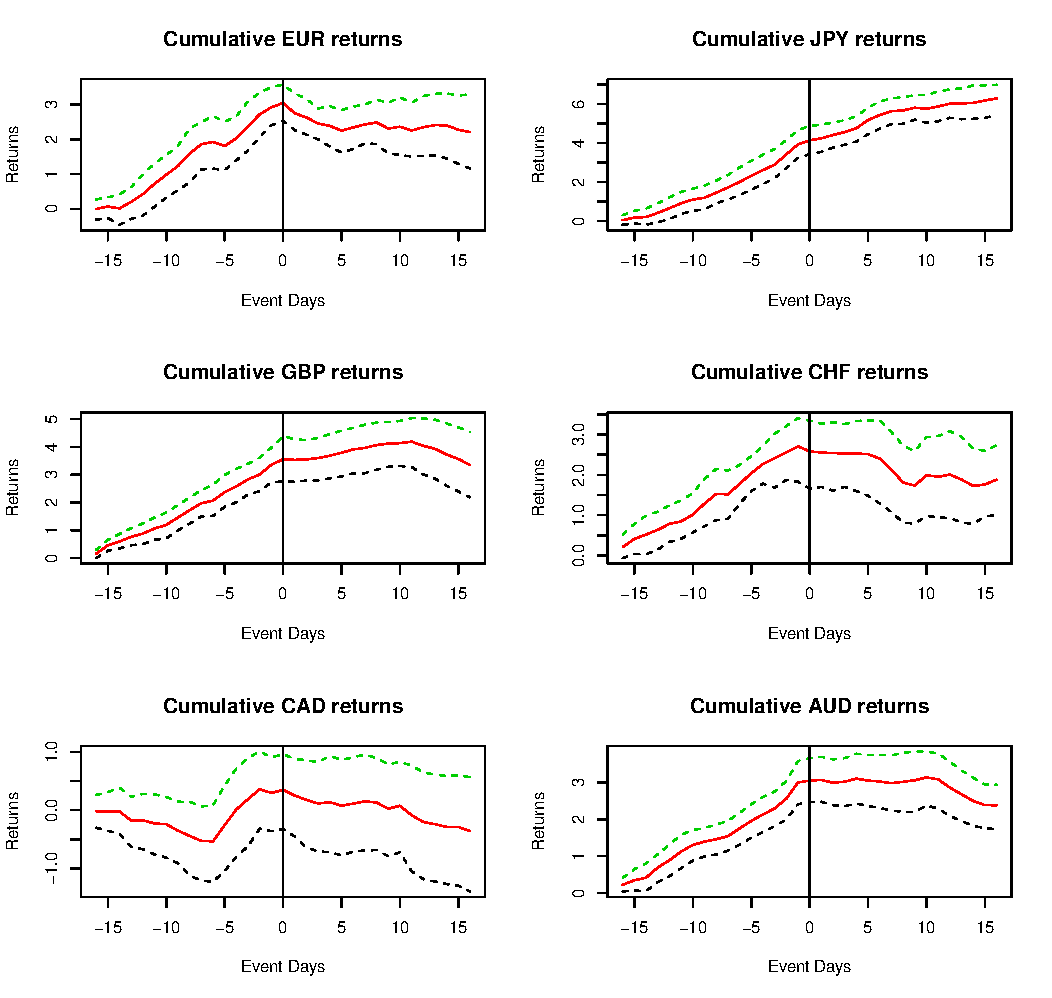
\includegraphics[scale=0.8]{RRCum16}
\caption{Event Study: Extreme (High $99{th}$ percentile) Risk Reversal Skew and 16 day event window: Risk reversals are the ratio of implied volatility on calls to the equivalent put; extreme high is at or above the $99^{th}$ percentile for the whole range, cumulative returns are the sum of log exchange rate returns. The event day is the day of the extreme risk reversal reading.  If speculation is uninformed, extremes should be followed by reversals; if speculation is informed, extremes are more likely to be followed by a random walk. The solid line is the cumulative mean return from the start of the event window; the dashed lines show the 95\% confidence intervals constructed from 1000 random bootstrap samples of appropriate event window day.}
\label{fig:ES5}
\end{figure}

\begin{figure}
\graphicspath{{../Figures/}}
\centering
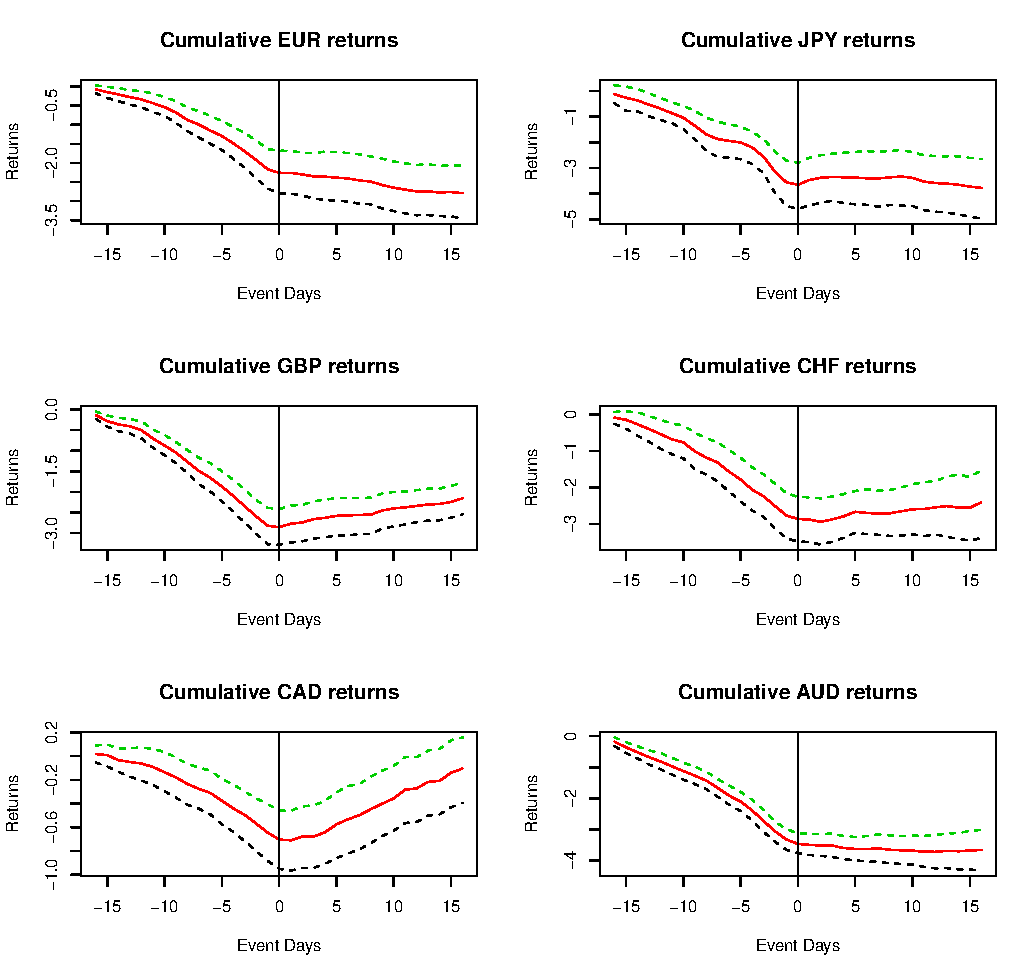
\includegraphics[scale=0.8]{RRCum16a}
\caption{Event Study: Extreme (Low $10{th}$ percentile) Risk Reversal Skew and 16 day event window: Risk reversals are the ratio of implied volatility on calls to the equivalent put; extreme low is at or below the $10^{th}$ percentile for the whole range, cumulative returns are the sum of log exchange rate returns. The event day is the day of the extreme risk reversal reading.  If speculation is uninformed, extremes should be followed by reversals; if speculation is informed, extremes are more likely to be followed by a random walk. The solid line is the cumulative mean return from the start of the event window; the dashed lines show the 95\% confidence intervals constructed from 1000 random bootstrap samples of appropriate event window day.}
\label{fig:ES2}
\end{figure}

Table \ref{tabref:SP1} shows the results from the event studies that were carried out using speculative positions as reported to US regulators.  The table works in a similar way to Table \ref{tabref:RR1}.  The first column is the exchange rate, defined as units per US dollar.  The table is then split into two parts.  The first part uses the S1 measure, the net non-commercial (speculative) positions relative to total non-commercial (speculative) positions; the second is S2 as the net non-commercial position relative to open interest or the total outstanding open positions.  Therefore, the first captures the balance of speculative positions while the second captures the balance of speculative positions relative to the whole market.  If speculators become more prevalent or dominant in the market, this will show up in S2 but not S1.  S1 is more sensitive to changes in sentiment and more volatile. Each of these sections is broken into the results for a 2 week window and a 4 week window.  There is a row for extreme high and extreme low which represents extreme long positions or extreme short positions; the first  column identifies the number of cases; CARW is the cumulative abnormal return for the whole event window; CARA is the cumulative abnormal return for the period after the event to the end of the window.     

\begin{sidewaystable}
% multirow package is required.   
%pdflandscape is required to facilitate the landscape position. 
\begin{threeparttable}
\caption{Event Study: Cumulative Abnormal Returns and Extreme Speculative Positions}
\begin{tabular}{llccccccccccccc}	
 % \hline
& &\multicolumn{6}{c}{S1 - Net Long per Speculators} & \multicolumn{1}{c}{} & \multicolumn{6}{c}{S2 -Net Long per Open Positions}\\
 & &\multicolumn{3}{c}{2 week} & \multicolumn{3}{c}{4 week} & \multicolumn{1}{c}{} & \multicolumn{3}{c}{2 week} & \multicolumn{3}{c}{4 week} \\ 
%\cline{4 - 10} \cline{13 - 19}
& &\multicolumn{1}{ c}{N} & \multicolumn{1}{c}{CARW} & \multicolumn{1}{c}{CARA} & \multicolumn{1}{ c}{N} & \multicolumn{1}{c}{CARW} & \multicolumn{1}{c}{CARA} & \multicolumn{1}{c}{} & 
\multicolumn{1}{ c}{N} & \multicolumn{1}{c}{CARW} & \multicolumn{1}{c}{CARA}  
& \multicolumn{1}{ c}{N} & \multicolumn{1}{c}{CARW} & \multicolumn{1}{c}{CARA}  \\   
\hline
\multirow{2}{*}{EUR} 
& Hi &  27 &  2.9415* & 1.3163* &27 & 3.8059* & 1.7341* &&27 & 1.0974* & 0.2896 &27 & 1.7667*& 0.0419  \\ 
& Lo & 27 & -2.4258* & -1.2512* & 27 &-3.9235* &-1.9254* & & 27 & -2.5122* & -1.0607* & 27 & -4.4478* & -1.9285* \\
\multirow{2}{*}{JPY}
& Hi & 43 & 1.9749* & 0.7286* & 43 & 2.8628* & 0.7909 & & 43 & 2.2463* & 1.0554* &43 & 3.7125* & 1.4443*  \\ 
& Lo & 43 & -2.2014* & -1.1312* & 43&-3.2488* & -1.5758* & &43 & -2.0605* & -0.9791* &43  & -2.6865* & -0.8318  \\
\multirow{2}{*}{GBP}
& Hi & 43 & 0.7102 & -0.2116 &43 & 1.0172* & -0.7902* & &43 & 1.2916* & 0.2370 &43 &1.6912* &0.0126  \\ 
& Lo & 43 &-0.6979* &0.2902 &43 &-1.5330* &0.1014 & &43 &-1.8993* &-0.1415 &43 &-2.8830* & -0.0768 \\
\multirow{2}{*}{CHF}
& Hi & 43 & 1.4400* & -0.0988 & 43 & 2.8665* & -0.0993 & & 43 &  2.5260* &  0.5074 & 43 & 3.6060* & 0.2158  \\ 
& Lo & 43 & -2.1816* &  -0.9770* & 43 &-3.3030* & -0.09798* & & 43 & -1.2605* & -0.3070& 43 &-0.1.6021* & 0.0670  \\
\multirow{2}{*}{CAD}
& Hi & 43 & 1.8658* & 1.0195* & 43 & 3.5298* & 1.8319* & & 43 & 2.0160* & 0.8788* &43 & 3.0995* & 0.9921*  \\ 
& Lo & 43 &-1.3238* & -0.5548* & 43 & -1.9151* & -0.7859* & & 43 & -1.2462* & -0.4505*  &43 & -1.9390*  & -0.6195*  \\
\hline
\label{tabref:SP1}
\end{tabular}
\begin{tablenotes}
\small 
\item Where Hi means extreme high, either S1 which is the measure of net long non-commercial (speculative) positions per total of speculators) or S2 which is the measure of net long non-commercial (speculative) positions per open interest (total outstanding open positions); high and low are above the $95^{th}$ percentile or below the $5^{th}$ percentile respectively; CARW is the cumulative abnormal return for the whole window, before and after the extreme event, and CARA is the cumulative abnormal return for the period after the event, which is the event day and the window; abnormal return is anything that is different from zero; the asterisk denotes significantly different from zero, where statistical significance is that more than 95\% of 1000 means calculated from random bootstraps from the extreme readings are above or below zero.   
\end{tablenotes}	
\end{threeparttable}  
\end{sidewaystable}

Once again, there is a very strong association between returns and the activity of speculators.  For the 4-day window and the S1 and S2 measures, every one of the currencies studied, high and low, had a mean cumulative return for the whole of the event window that was in the same direction as sentiment.  When re-sampled a thousand times, more than ninety five percent of the means calculated were greater than zero in all cases but one (GBP).  There is evidence here of momentum and of prices following the movement of speculator positions. 

\begin{figure}
\graphicspath{{../Figures/}}
\centering
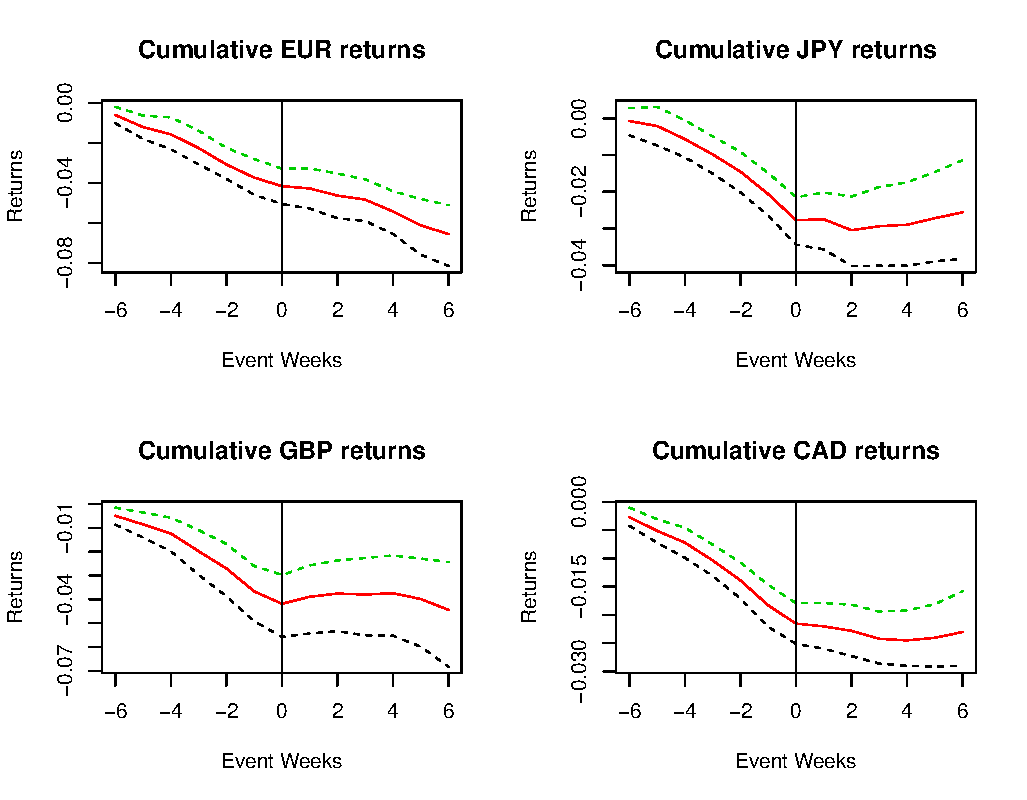
\includegraphics[scale=0.8]{FPCum6w}
\caption{Event Study:  Extreme ($90^{th}$ percentile), Non-commercial net long (S1), 6 week window. Non-commercial net per OI (S2) are the net speculative positions (as reported to US regulator the CFTC) relative to all open positions; extreme high is at or above the $90^{th}$ percentile for the whole range, cumulative returns are the sum of log exchange rate returns. The event day is the day of the extreme reading as a measure of extreme speculative activity.  If speculation is uninformed, extremes should be followed by reversals; if speculation is informed, extremes are more likely to be followed by a random walk.}
\label{fig:ES3}
\end{figure}

\begin{figure}
\graphicspath{{../Figures/}}
\centering
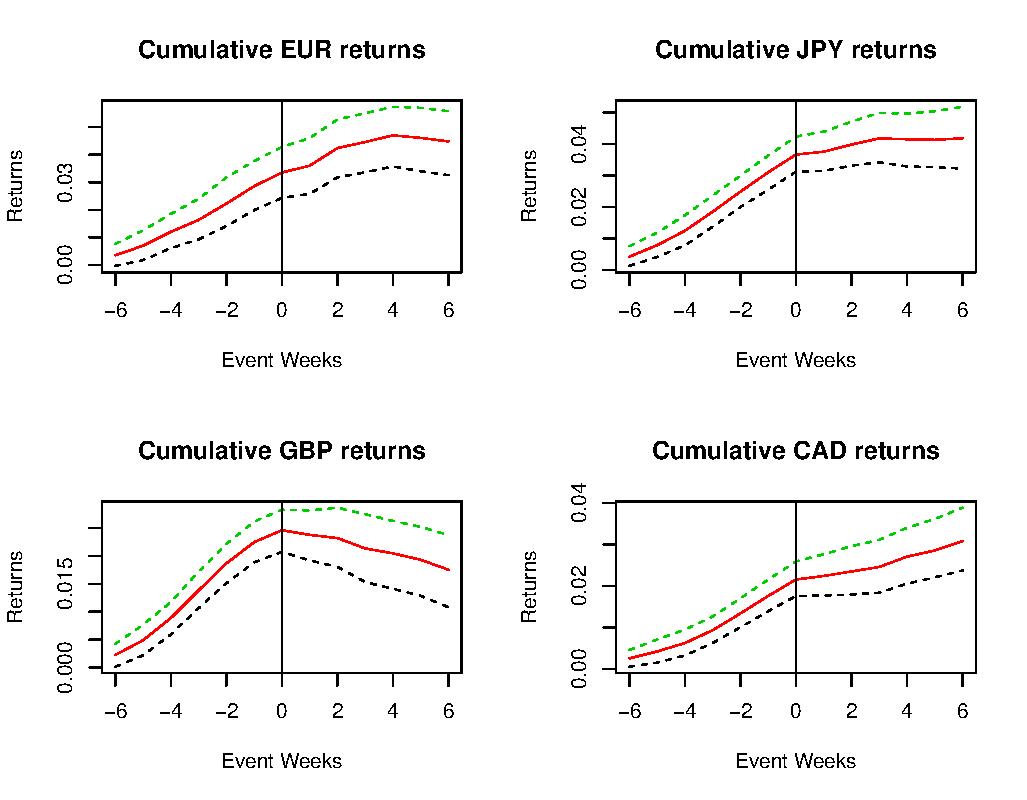
\includegraphics[scale=0.8]{FPCum6wa}
\caption{Event Study:  Extreme ($90^{th}$ percentile), Non-commercial net long (S1), 6 week window. Non-commercial net per OI (S2) are the net speculative positions (as reported to US regulator the CFTC) relative to all open positions; extreme high is at or above the $90^{th}$ percentile for the whole range, cumulative returns are the sum of log exchange rate returns. The event day is the day of the extreme reading as a measure of extreme speculative activity.  If speculation is uninformed, extremes should be followed by reversals; if speculation is informed, extremes are more likely to be followed by a random walk.}
\label{fig:ES4}
\end{figure}

There is little evidence that these self-reported speculators are driving prices away from fundamentals with their activity. Sixty percent of the S1 cases still show a significant abnormal return in the direction of the extreme 4 weeks after the extreme has been reached; only thirty percent of the cases show a reversal and in only one of those do ninety five percent of the means calculated after re-sampling remain above zero.  For S2 there is even less clarity, with ninety percent of the cases showing a continuation and forty percent of them showing significant continuation.  The evidence here with speculative positions is the same as that of speculative sentiment.  Prices move in the direction of speculative activity but speculative extremes do not provide information about the future. The price action of the event study is consistent with speculation being informed rather than uninformed.  Figures \ref{fig:ES3} and \ref{fig:ES4} show a selection of event studies that were carried out.  Figure \ref{fig:ES3} is the extreme low ($10^{th}$ percentile) with a 13 week window. There is no evidence of a reversal in any of the currency units.   Figure \ref{fig:ES4} is the extreme high ($90^{th}$ percentile) with a 13 week event window.  Only the GBP shows any evidence of reversal. It is not statistically significant. 


\section{Speculation and foreign exchange returns}
If foreign exchange speculation is uninformed noise, extreme speculation, whether measured by sentiment or weight of activity, will coincide with deviations from fundamental value; if speculation is informed, speculation is part of the process of price discovery and extremes will provide no information about future prices. An event study showed that speculation is associated with price movement: exchange rates move in the direction of speculative sentiment and activity.  However, once extreme \added{speculative sentiment or extreme speculative positions are established}, prices are as likely to continue as to reverse. Speculative sentiment and speculative activity influence foreign exchange prices as indicated by the covariance of speculative measures with returns.  These results show that foreign exchange speculation is an important part of the price discovery process.  The random walk after the extreme is indicative of foreign exchange prices absorbing most of the information that is available.  
  
The results are not a function of the design of the event study.  The event window and the quantiles that are chosen to measure the extreme can be changed.  Alternative measures produced very similar results. Alternative quantiles from 1\% and 99\% to 20\% and 80\% have been assessed; Figures \ref{fig:ES1}, \ref{fig:ES2}, \ref{fig:ES3} and \ref{fig:ES4} have much wider windows and do not find any alternative to the view that extreme speculation is followed by a random walk. 

It is encouraging that two very different measures of speculative activity produce very similar results and that the results hold over different time frames: one week for the option data and one week for the regulatory position data.  It is less clear whether the results would be reproduced across markets for other financial assets. \added{The foreign exchange market has a particular microstructure that is dominated by over-the-counter transactions in the spot market and this may influence the results.  Further reseach might look at risk-reversals in financial markets that are traded on electronic exchanges to see if these results are replicated.  The data on speculative positions are from the excahnge traded futures market.} \deleted{The results do not rule out uninformed speculation.  The Friedman effect from the Noise-trader model, whereby the informed speculators take advantage of the space created by price pressure from the uniformed, depends on there being \emph{noise-trader risk} or some limits to arbitrage.  The effect is not evident in this study.}  However, the foreign exchange market is a particularly large and liquid market, other asset classes may have alternative institutional features that mean a different relationship or balance between the informed and uninformed and therefore different results.  

\added{It is possible to dispute the link between risk reversal and market sentiment. It is not only the direct change in expectations about the future that affect  risk-reversals. The weight of positions from hedging activity could be influential. Therefore future research might also investigate the link between these figures and other measures of short-term sentiment if they exist.}
\deleted{This is important because there is no unambiguous view of speculative activity and because speculation is an important issues in a number of policy debates.  Most notably, the \emph{Tobin Tax} would put a charge against financial transactions, particularly in foreign exchange.  Part of the argument depends on speculation being uninformed as the reduced activity that is caused by the tax would, it is argued, limit volatility and allow more long-term fundamental evaluations to become prominent.  However, if speculation is informed and part of the price discovery process, this tax may have the opposite effect to what is envisaged.  These results suggest that it could reduce liquidity and increase volatility.} 



%=====================================
% References, variant B: external bibliography
%=====================================
\externalbibliography{yes}
\bibliography{myrefs}

%%%%%%%%%%%%%%%%%%%%%%%%%%%%%%%%%%%%%%%%%%
%% optional
%\sampleavailability{Samples of the compounds ...... are available from the authors.}

%%%%%%%%%%%%%%%%%%%%%%%%%%%%%%%%%%%%%%%%%%
\end{document}

